\chapter{Methodology}
\label{chapter:methodology}

This section begins by defining the phases that constitute the research. Following that, it outlines the beginning of the design of the system's structure by defining its architecture, features, and workflows. To meet the acceptance criteria for this stage and take into account the volume of this research, a strategic framework was selected to guide the architectural design of the proposed solution. Using \ac{acdm} principles and methodology, this chapter defines the solution's initial requirements, stakeholders, challenges and architecture.

% ____________________ Phases of the Research ____________________ %

\section{Phases of the Research} \label{section:phases_of_the_research}

To realise the previously mentioned objectives, the proposed research can be conducted in four key stages, which align with a logical progression from understanding the problem to focusing on different aspects of design and development.

\begin{outline}[enumerate]
    \1 Study the State-of-the-Art and identify design approaches:
        \2 Review existing;
        \2 \aclp{lfms};
        \2 In-production solutions;
        \2 Available and recommended technologies;
        \2 Best practices and optimal approaches;
    \1 Design the structure of the system by defining its architecture, features and workflows;
    \1 Create the main system components, including all the planned features;
    \1 Test the system in a real-world and controlled environment;
    \1 Finalise and document the results for academic and practical use.
\end{outline}

% ____________________ Architecture-Centric Development Methodology ____________________ %

\section{\acl{acdm}} \label{section:acdm}

The \ac{acdm} is a software development methodology, mainly inspired by Quality Attribute Workshop, Architecture Tradeoff Analysis Method and Attribute Driven Design, that emphasises the use of software architecture as a primary driver for the development process \cite{Lattanze2005}. It integrates architectural design into the overall lifecycle of software development, aiming to improve quality, predictability, and efficiency. Below are the key aspects of \ac{acdm} based on the provided paper. \ac{acdm} is structured around the concept that software architecture serves as the backbone of the system, providing a framework for ensuring consistency, scalability, and alignment with business goals. The architecture is not only a technical construct but also a means of communication among stakeholders.

% ____________________ Definition ____________________ %

\subsection{Definition}

As shown in Figure \ref{fig:acdm_workflow}, the \ac{acdm} organises the architectural design process into clearly defined stages that evolve iteratively. \ac{acdm} is inherently iterative, with the flexibility to revisit earlier stages based on findings or changing requirements.

\begin{figure}[!htb]
    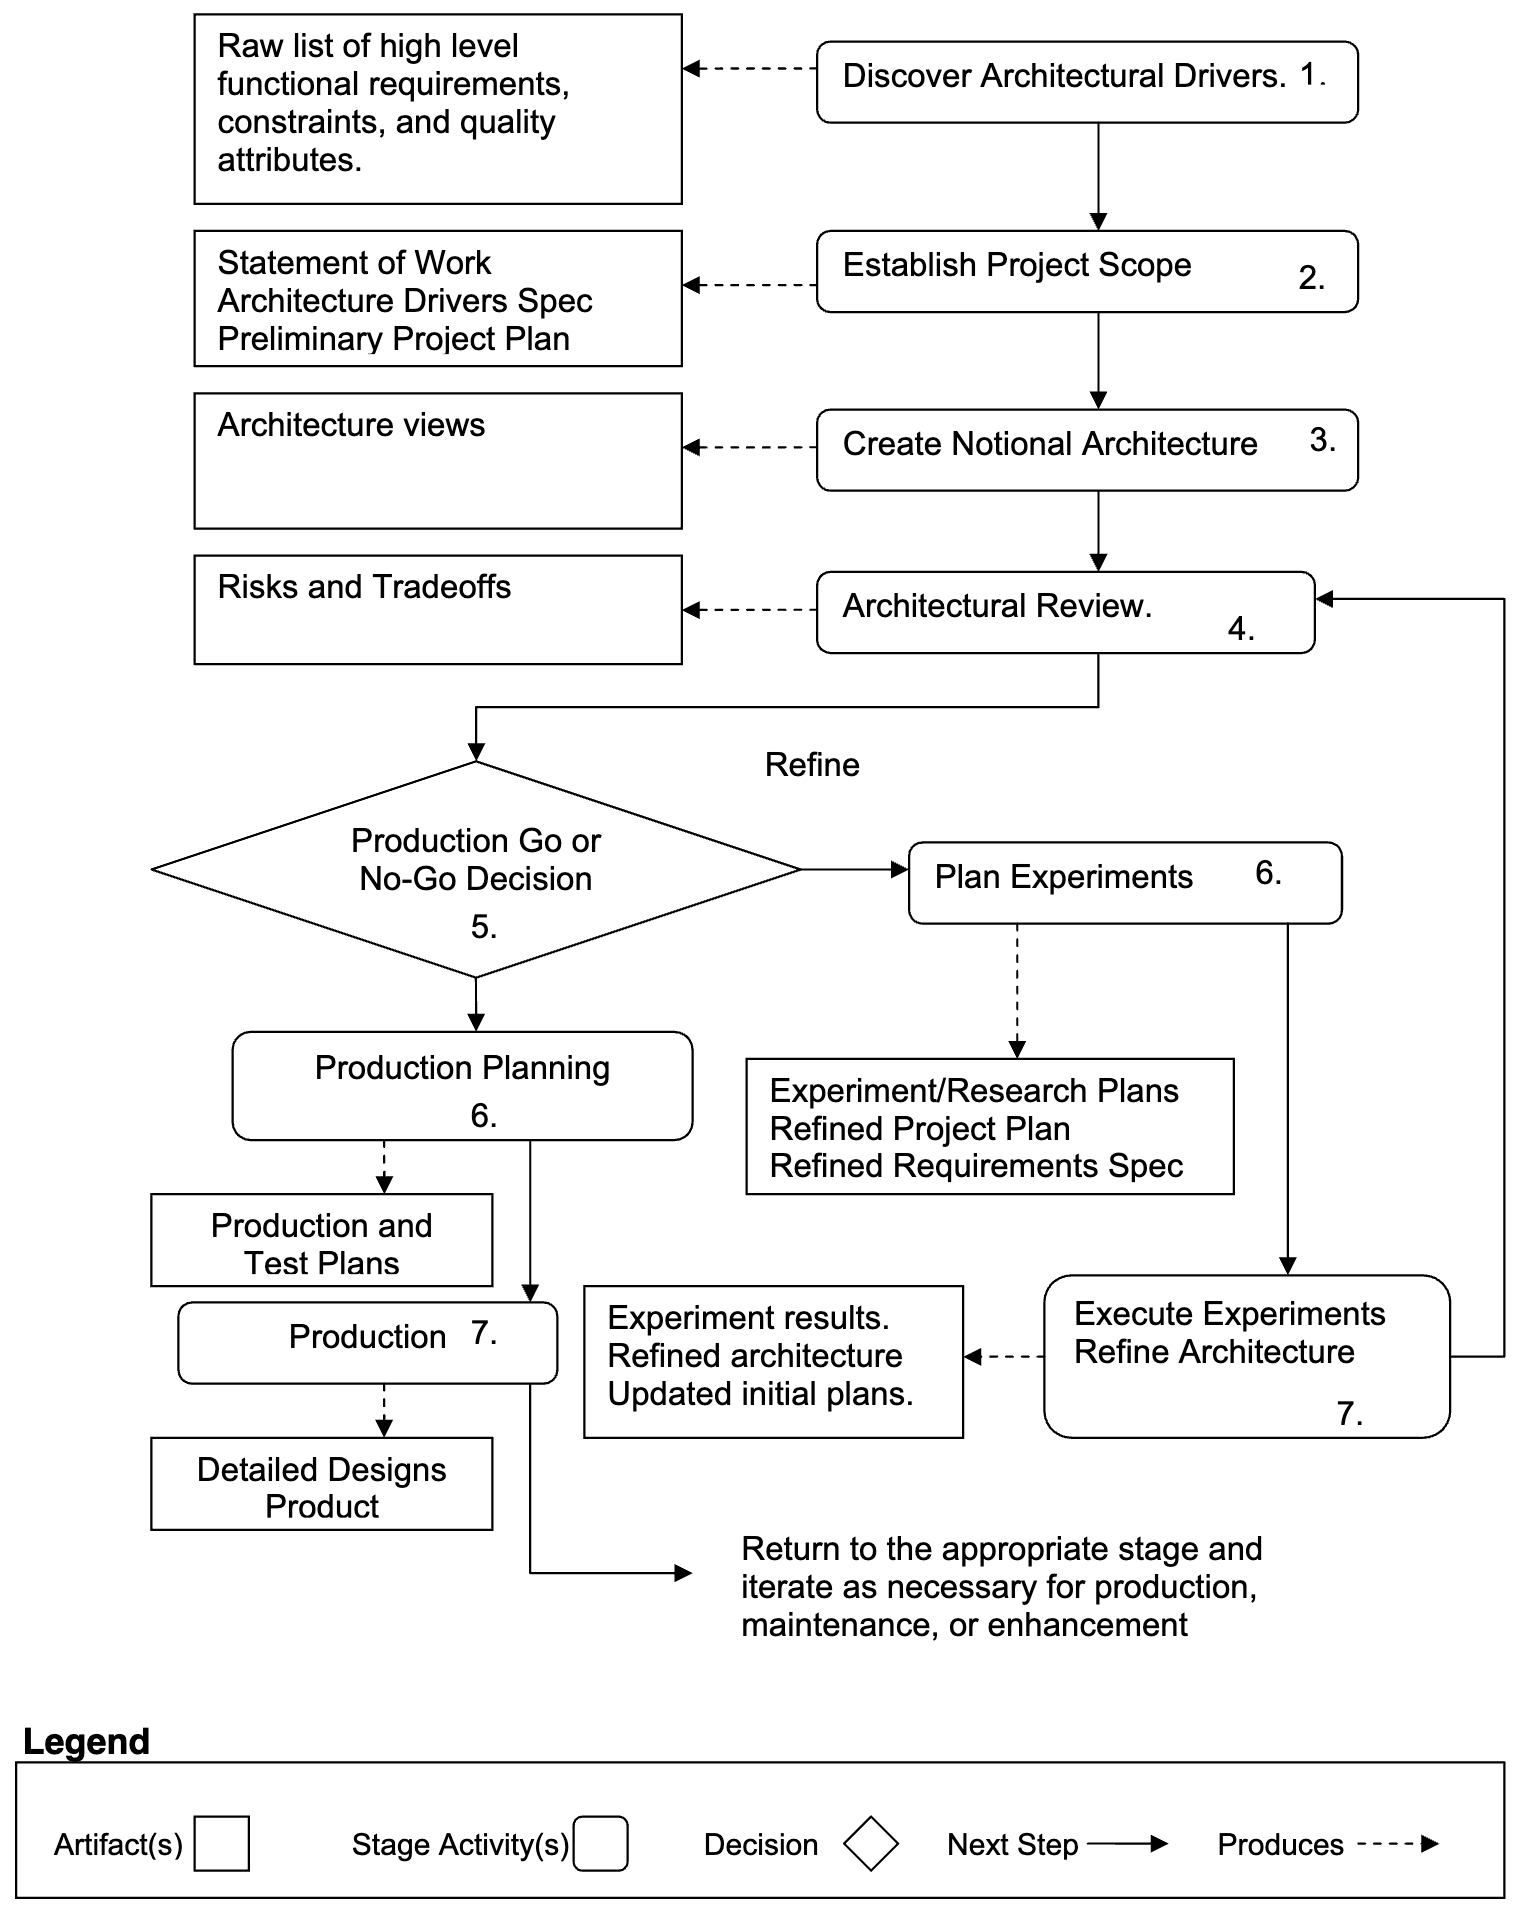
\includegraphics[width=0.6\textwidth]{figs/chapter3/acdm_workflow.png}
    \centering
    \caption[\acl{acdm} Workflow]{\ac{acdm} workflow, illustrating the iterative stages, the flow of artifacts, decisions, and refinements through the development process. Adapted from \citeauthoryear{Lattanze2005}.}
    \label{fig:acdm_workflow}
\end{figure}

\subsubsection{Architectural Drivers}

According to \citeauthoryear{Lattanze2005}, the process begins with discovering the architectural drivers, where crucial factors such as functional requirements, quality attributes (e.g., performance, scalability, security), and constraints are identified. These drivers form the foundation for all subsequent design decisions. Appendix \ref{app:architectural-design} contains the remaining stages of the \ac{acdm} process, which provide a fully defined set of the architectural drivers for this research.

\subsubsection{Project Scope}

Following this, the project scope is established to define the system's boundaries, objectives, deliverables, and constraints, ensuring that all stakeholders have a shared understanding of the project's limits and expectations.

\subsubsection{Notional Architecture}

Once the drivers and scope are defined, a notional architecture is created as a high-level conceptual design. This step involves decomposing the system into components, defining their responsibilities, interactions, and dependencies, and adopting appropriate architectural styles and patterns. The notional architecture serves as a blueprint for early-stage validation.

\subsubsection{Architectural Review}

The design is then subjected to an architectural review, where it is assessed against the architectural drivers and project scope. Scenario-based evaluations, risk assessments, and stakeholder feedback are key activities during this stage. The outcome is a decision to either proceed to production or refine the architecture further.

\subsubsection{Refinement Phase}

If the architecture is deemed insufficient during the review, the process enters a refinement phase. This phase begins with the \textbf{experiment planning}, where targeted experiments are designed to address specific weaknesses or uncertainties, such as performance bottlenecks or scalability challenges. These experiments are executed in the \textbf{experiment execution} and subsequent \textbf{architecture refinement} stage, with findings informing updates to the architecture. Once refined, the updated architecture undergoes another review to ensure it meets the required standards before moving forward.

\subsubsection{Production Phase}

If the architecture passes the review, the process transitions to the production phase, beginning with the \textbf{production planning}, which involves preparing the system for deployment by developing detailed plans, establishing monitoring mechanisms, and guaranteeing operational readiness. Finally, the system is deployed during the \textbf{production} stage, when it becomes operational and accessible to end-users. Post-deployment, the architecture is continuously monitored for performance and feedback, allowing iterative improvements as needed.

% ____________________ Quality Attributes ____________________ %

\subsection{Quality Attributes} \label{section:quality_attributes}

The quality attributes form the foundation for platform development. These attributes were selected based on their priority for solution success and their relevance to the key challenges identified in the problem domain.

\subsubsection{Scalability}

The platform must accommodate a growing user base and increased item-tracking demands across diverse locations. A microservices architecture is proposed to enable independent scaling of critical system components, such as user management and item management \cite{Al-Debagy2021}. This scalability aligns with the goal of creating a community-oriented system capable of handling high-traffic scenarios and fluctuations in demand without compromising performance.

\subsubsection{Reliability} 

Consistent performance is essential, even in adverse conditions like network failures. Reliable performance builds user trust, which is fundamental to any lost property management system. Fault-tolerant mechanisms, including distributed databases and redundant servers, will ensure high availability (targeting 99\% uptime) and minimize the "mean time to repair"\footnote{\url{https://www.atlassian.com/incident-management/kpis/common-metrics}}. Automated monitoring and self-healing protocols will detect and address faults proactively.

\subsubsection{Security}

Handling sensitive data, such as user information and potentially high-value lost items, requires a security-first approach. Security measures further reinforce the platform's reliability and address concerns like identity theft and elevated access, two key pain points identified in this research. End-to-end encryption for secure authentication and granular authorisation mechanisms will protect data privacy. Due to the sensitivity of the data the system is going to handle, it is obliged to adhere to \ac{gdpr}\footnote{\url{https://gdpr-info.eu/}} and other relevant regulations to ensure the lawful handling of personal information.

\subsubsection{Usability}

The system targets a broad spectrum of users, including non-technical individuals, requiring an intuitive and accessible interface. Following \ac{ui} and \ac{ux} best practices with ongoing feedback loops will support iterative platform improvements. Multilingual support and visual guidance will also cater to diverse user demographics.

\subsubsection{Observability}

Incorporating observability tools to collect logs, metrics, and traces will allow real-time and long-term monitoring of the system's performance and user interactions \cite{Niedermaier2023}. Observability also allows quick detection and resolution of operational issues, providing insights for continuous improvement.

% ____________________ Requirements ____________________ %

\subsection{System Requirements} \label{section:requirements}

The system's design and implementation are guided by its requirements, which can also be used to measure the research progress and value. When correctly specified, they help the developer understand the expected result, and the stakeholders evaluate the system's performance. These requirements fall into two categories: functional and non-functional. Table \ref{tab:functional_requirements} lists the functional requirements that define the core features of the system, focusing on enabling users to interact with and manage data effectively.

\begin{table}[!htb]
\centering
\begin{tabular}{|p{0.1\textwidth}|p{0.80\textwidth}|}
\hline
\textbf{ID} & \textbf{Functional Requirement Description} \\ \hline
FR1 & Support three user roles: ordinary users, local managers, and administrators. \\ \hline
FR2 & Enable secure account management for all user types. \\ \hline
FR3 & Implement authentication and authorization mechanisms, including multi-factor authentication. \\ \hline
FR4 & Allow users to browse and search lost items based on categories and filters (e.g., location, type). \\ \hline
FR5 & Provide personalized suggestions for matching items using \ac{ai}. \\ \hline
FR6 & Facilitate item status updates and notifications to users about item matches or updates. \\ \hline
FR7 & Enable users to schedule appointments for item retrieval. \\ \hline
FR8 & Allow administrators to audit system logs and manage user roles effectively. \\ \hline
FR9 & Integrate community-driven features for collaborative lost item recovery. \\ \hline
\end{tabular}
\caption[Functional Requirements]{Functional requirements defining the core system features.}
\label{tab:functional_requirements}
\end{table}

On the other hand, Table \ref{tab:nonfunctional_requirements} presents the non-functional requirements, which are directly connected with the system's expected quality levels.

\begin{table}[!htb]
\centering
\begin{tabular}{|p{0.1\textwidth}|p{0.80\textwidth}|}
\hline
\textbf{ID} & \textbf{Non-Functional Requirement Description} \\ \hline
NFR1 & Ensure a response time of less than 2 seconds for critical operations under peak load. \\ \hline
NFR2 & Support scalability to accommodate up to 10,000 concurrent users. \\ \hline
NFR3 & Comply with data privacy regulations such as \ac{gdpr}. \\ \hline
NFR4 & Maintain 99\% uptime through fault tolerance and disaster recovery mechanisms. \\ \hline
NFR5 & Adhere to \ac{ux} and \ac{ui} best practices. \\ \hline
NFR6 & Implement modular and extensible architecture for easier updates and debugging. \\ \hline
NFR7 & Incorporate monitoring tools for real-time performance tracking and troubleshooting. \\ \hline
NFR8 & Secure compatibility across devices. \\ \hline
\end{tabular}
\caption[Non-Functional Requirements]{Non-functional requirements defining the system's quality attributes.}
\label{tab:nonfunctional_requirements}
\end{table}


% ____________________ Constraints ____________________ %

\subsection{Constraints} \label{section:constraints}

The development of the system is governed by two primary constraints that shape its scope, deliverables, and quality:

\subsubsection{C1: Timeframe Limitation}

The development is restricted to a 10-month timeframe in which it is embedded.

\subsubsection{C2: Verifiable Quality}

Both software and design quality must be verifiable, meaning the stakeholders must test the system and review its code.

% ____________________ Notional Architecture ____________________ %

\section{Notional Architecture} \label{section:notional_architecture}

As previously mentioned, the architecture is iteratively refined. The initially proposed architecture, visible in Figure \ref{fig:initial_arch}, was designed as a microservices-based system, dividing the application into distinct, independent services, each responsible for a specific functionality \cite{Al-Debagy2021,Söylemez2024}. This planned architecture grouped the system's components into three main layers: the frontend, backend, and support infrastructure, as follows:

\begin{figure}[!htb]
    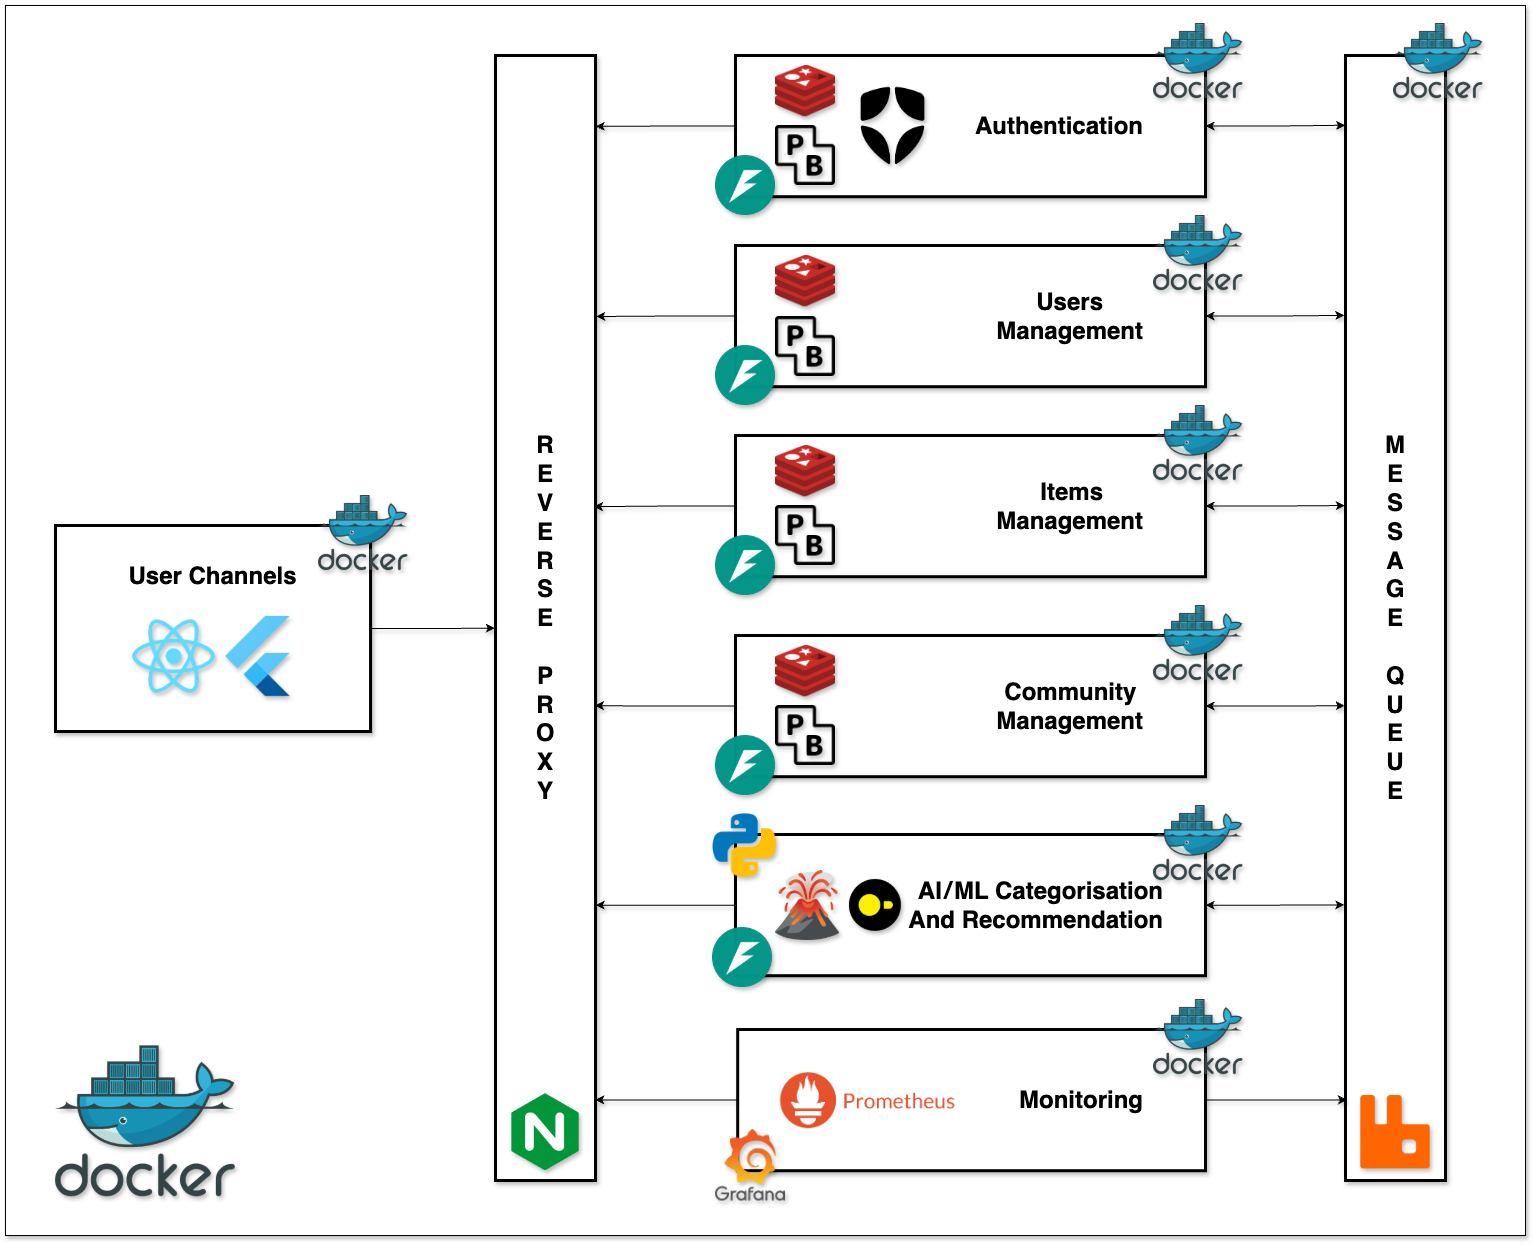
\includegraphics[width=0.8\textwidth]{figs/chapter3/initial_arch.png}
    \centering
    \caption[Initial Microservices Architecture]{High Level View of the Initially Planned Microservices Architecture.}
    \label{fig:initial_arch}
\end{figure}

\subsection{Frontend}

The frontend provides users with a seamless and intuitive interface for both web and mobile platforms, enabling easy access to all system features and smooth interaction with the backend services.

\subsection{Initial Backend Architecture}

The backend was initially designed as a collection of microservices that would provide distinct functionalities across the system. The Authentication Service was planned to handle user authentication and authorisation through role-based access control, securing controlled access to the system. A dedicated Users Management Service would manage user profiles, including registration and updates, ensuring comprehensive user lifecycle management. The Items Management Service was conceived as the core service of the system, focusing on fetching, storing and updating lost items while integrating with other services to provide seamless item tracking and retrieval functionalities. Additionally, a Community Management Service was designed to handle direct communication between ordinary users and the chat spaces available for each community, fostering collaborative recovery efforts. Finally, an AI/ML Categorization and Recommendation Service was planned to automatically identify and categorise items based on images and descriptions, processing user inputs and interactions to actively match and recommend items to ordinary users searching for lost property.

\subsubsection{Initial Support Infrastructure}

The infrastructure was planned to provide the foundation for deploying and managing the microservices system through several key components. A reverse proxy was designed to route incoming requests to the appropriate services, providing load balancing and enhancing the system's overall security by handling HTTPS termination. The architecture also included a message queue system that would facilitate asynchronous communication between microservices, ensuring that each service operates independently even during periods of high data throughput. Furthermore, a comprehensive monitoring solution was planned to collect performance metrics and provide dashboards for real-time visualisation of system health and performance indicators.

% ____________________ Technology Stack ____________________ %

\subsection{Proposed Technologies to be Used}

The selection of technologies is based on their alignment with the architectural drivers and the system's requirements. The proposed technology stack is as follows:

For the frontend, React\footnote{\url{https://react.dev/}} will be used to build a dynamic and interactive web application, mainly for administrative uses inside the platform. At the same time, Flutter will enable cross-platform mobile application development, ensuring an accessible and consistent user experience across locations and devices.

The backend was planned to be essentially powered by FastAPI\footnote{\url{https://fastapi.tiangolo.com/}}, a Python\footnote{\url{https://www.python.org/}}-based framework that excels at building high-performance \acp{api} for small/medium projects, with the main purpose of supporting asynchronous operations. Authentication was planned to be secured using OAuth 2.0\footnote{\url{https://oauth.net/2/}}, a widely adopted protocol, that would be capable of granting and managing secure access and role-based access control. The system was planned to rely on Pocketbase\footnote{\url{https://pocketbase.io/}}, an open-source Backend-as-a-Service, for handling database operations and real-time data sync, complemented by Redis\footnote{\url{https://redis.io/}} for caching and session management, in order to guarantee fast data access and reduce the backend load. For \ac{ai}-driven functionalities, \ac{llava}\footnote{\url{https://llava-vl.github.io/}}, an end-to-end trained large multimodal model, would combine language and vision processing. Data analytics was planned to be supported by DuckDB\footnote{\url{https://duckdb.org/}}, an in-process analytical database that would efficiently process the complex embeddings generated by \ac{llava}. Considering the necessity of valuable monitoring, Prometheus\footnote{\url{https://prometheus.io/}} would collect metrics across the system, and, using Grafana\footnote{\url{https://grafana.com/}}, would enable intuitive dashboards for real-time visualisation and performance tracking. 

The entire infrastructure was planned to be containerised using Docker\footnote{\url{https://www.docker.com/}}, ensuring consistency across environments and simplifying deployment. Nginx\footnote{\url{https://nginx.org/en/}} would act as a reverse proxy and load balancer, enhancing request routing. Finally, RabbitMQ\footnote{\url{https://www.rabbitmq.com/}} would serve as the unique message broker, enabling asynchronous and reliable communication between the microservices.

% ____________________ Architectural Evolution ____________________ %

\section{Architectural Evolution and Implementation Reality} \label{section:architectural_evolution}

During the development process, several constraints and practical considerations necessitated an evolution from the initially planned microservices architecture to a more pragmatic implementation approach.

\subsection{Development Constraints and Reality Assessment}

The transition from the planned microservices architecture was driven by several critical constraints that became apparent during the initial development phases. The limited development timeline, combined with the solo developer context, created significant constraints on the complexity of infrastructure that could be realistically implemented and supported.

Research indicates that microservices architectures introduce significant infrastructure overhead, with each new microservice requiring its own test suite, deployment playbooks, hosting infrastructure, and monitoring tools, leading to exponential infrastructure costs \cite{ServiceCostOverhead2023}. Studies comparing monolithic and microservice architectures show that microservices can require 4.22x more runtime processing time and exhibit 2.69x more overhead in Java EE applications \cite{MonolithicVsMicroservices2020}. In the context of academic dissertation evaluation, the primary focus is on demonstrating problem-solving capabilities, domain knowledge, and feature completeness rather than infrastructure complexity. The microservices approach, while architecturally sophisticated, would divert resources from delivering a functional system with comprehensive features or even a minimum viable product.

The planned microservices architecture would require managing 9+ separate services, databases, and deployment pipelines, which, for a solo developer, represents a significant operational burden that could compromise system reliability and long-term viability within the project timeline.

% TODO: Add figure showing the final implementation architecture here

\subsection{Final Implementation Architecture}

Based on the constraint analysis, the system was implemented using a modular monolithic architecture that preserves microservices design principles while consolidating deployment and operational complexity.

The system uses a single FastAPI application implementing a Router-Service-Repository pattern, which provides clear domain boundaries equivalent to microservices while preserving operational simplicity. The API incorporates an integrated authentication system that combines user authentication and authorization with role-based access control for three distinct user types: ordinary users, local managers, and system administrators. A unified item management approach consolidates item \ac{crud} operations, status tracking, and AI-powered matching within a cohesive service layer, ensuring seamless data flow and consistency. The system embeds community features by integrating real-time communication and community management as internal modules, preserving the collaborative aspects without requiring separate service deployment. Additionally, internal queue processing implements asynchronous operations using an internal queue system rather than external message brokers, reducing infrastructure complexity while preserving system responsiveness.

PocketBase serves as a unified data layer with real-time synchronization capabilities, eliminating the need for separate database management systems. Authentication is handled through PocketBase's built-in authentication system with JWT token management, providing secure and efficient user session management. AI integration utilizes the LLaVA model accessed through Ollama for multimodal processing, enabling intelligent item recognition, categorization, grouping, and matching. Nginx functions as the API gateway, providing security, SSL termination, and traffic management capabilities. System monitoring is achieved through Prometheus and Grafana for comprehensive performance tracking, while Docker and Docker Compose ensure consistent deployment across different environments.


% ____________________ Summary ____________________ %

\section{Summary} \label{section:methodology_summary}

This chapter has outlined the methodology used in developing the intelligent lost and found management system, showing how \ac{acdm} principles guided the design and implementation process. The research progressed through four distinct phases, from state-of-the-art analysis to system deployment and validation.

The methodology encompassed the identification of architectural drivers, including critical quality attributes such as scalability, reliability, security, usability, and observability, which guided all subsequent design decisions. The system requirements were systematically defined, establishing both functional capabilities and non-functional performance criteria that align with the identified challenges in lost property management.

A significant aspect of this methodology was the architectural evolution process, which demonstrated how theoretical design must adapt to practical constraints while preserving core architectural principles. The transition from the initially planned microservices architecture to a modular monolithic implementation was driven by a realistic assessment of development timeline and resource constraints, ensuring that the platform remained feasible within the academic context. Throughout this process, the preservation of scalability and modularity principles was prioritized to ensure opportunities for future system enhancement and, mainly, evolution.

The final implementation architecture successfully balances sophisticated functionality with operational simplicity, delivering a comprehensive system that addresses the identified research objectives while remaining within the leveraged constraints. This transformation demonstrates engineering maturity by prioritizing feature delivery and system reliability over infrastructure complexity. The Router-Service-Repository pattern employed ensures clear separation of concerns through well-defined service boundaries, enabling selective scaling or extraction when system growth demands it. Error containment mechanisms isolate failures at the domain level, preventing cascading issues across the entire application while establishing the foundation for future architectural evolution as system demands grow.

Additionally, this method provides a replicable framework for similar medium-sized academic and professional projects, demonstrating how architectural decisions should be guided by empirical analysis rather than purely theoretical considerations, ultimately resulting in more successful and sustainable software systems.
